\subsection{UC-10}
\label{subsec:UC-10}

\begin{figure}[H]
    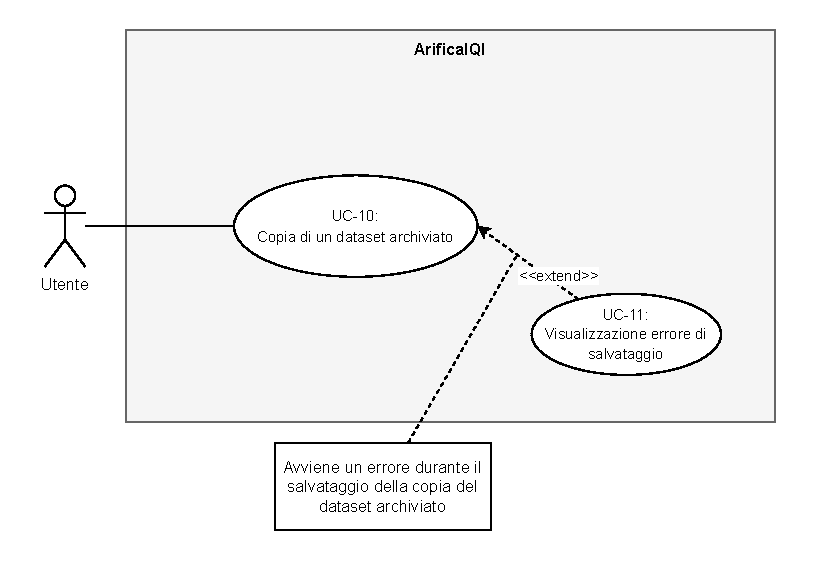
\includegraphics{Sezioni/UseCase/Immagini/UC-10.pdf}
    \caption{Diagramma UC-10.}
\end{figure}

\begin{usecase}{UC-10}{Copia di un dataset archiviato}
    \req{\hyperref[item:RU-3]{RU-3}} 

    \pre{
        \item Il sistema è attivo e funzionante
        \item Il dataset archiviato da copiare esiste
    }

    \post{
        \item Viene archiviata una nuova copia del dataset selezionato usando un nome di default
    }
    
    \actor{Utente}

    \subactors{}

    \trigger{L'utente deve creare una copia di un dataset precedentemente archiviato}
    
    \inc{}

    \base{}

    \scenario{
        \item L'utente richiede di copiare un dataset archiviato
        \item Viene salvata nel sistema una copia del dataset selezionato con un nome di default
    }

    \subscenario{
        \item[2.1] \textbf{Avviene un errore durante il salvataggio della copia del dataset}
        \begin{itemize}
            \item[a.] \hyperref[subsec:UC-11]{UC-11}
        \end{itemize}
    }

\end{usecase}